\subsection{Multiplikative Unsicherheit von \textit{T(s)}}
    Modellunsicherheit $W_2(s)$ ist multiplikativ für die komplementäre Sensitivität eingeführt. Dies führt zum \textit{robusten Nyquist Theorem:}
    \begin{equation*}
        |T(\jw)\cdot W_2(\jw)| < 1 \Rightarrow |L(\jw)\cdot W_2(\jw)| < |1+L(\jw)|
    \end{equation*}
    Im Bode-Plot kann man das relativ einfach überprüfen, indem man schaut ob folgende Ungleichung erfüllt ist.
    \begin{equation*}
        |T(\jw)| <  |W_2^{-1}(\jw)|
    \end{equation*}
    
    Man kann das wie folgt geometrisch interpretiern:
    \begin{figure}[H]
        \centering
        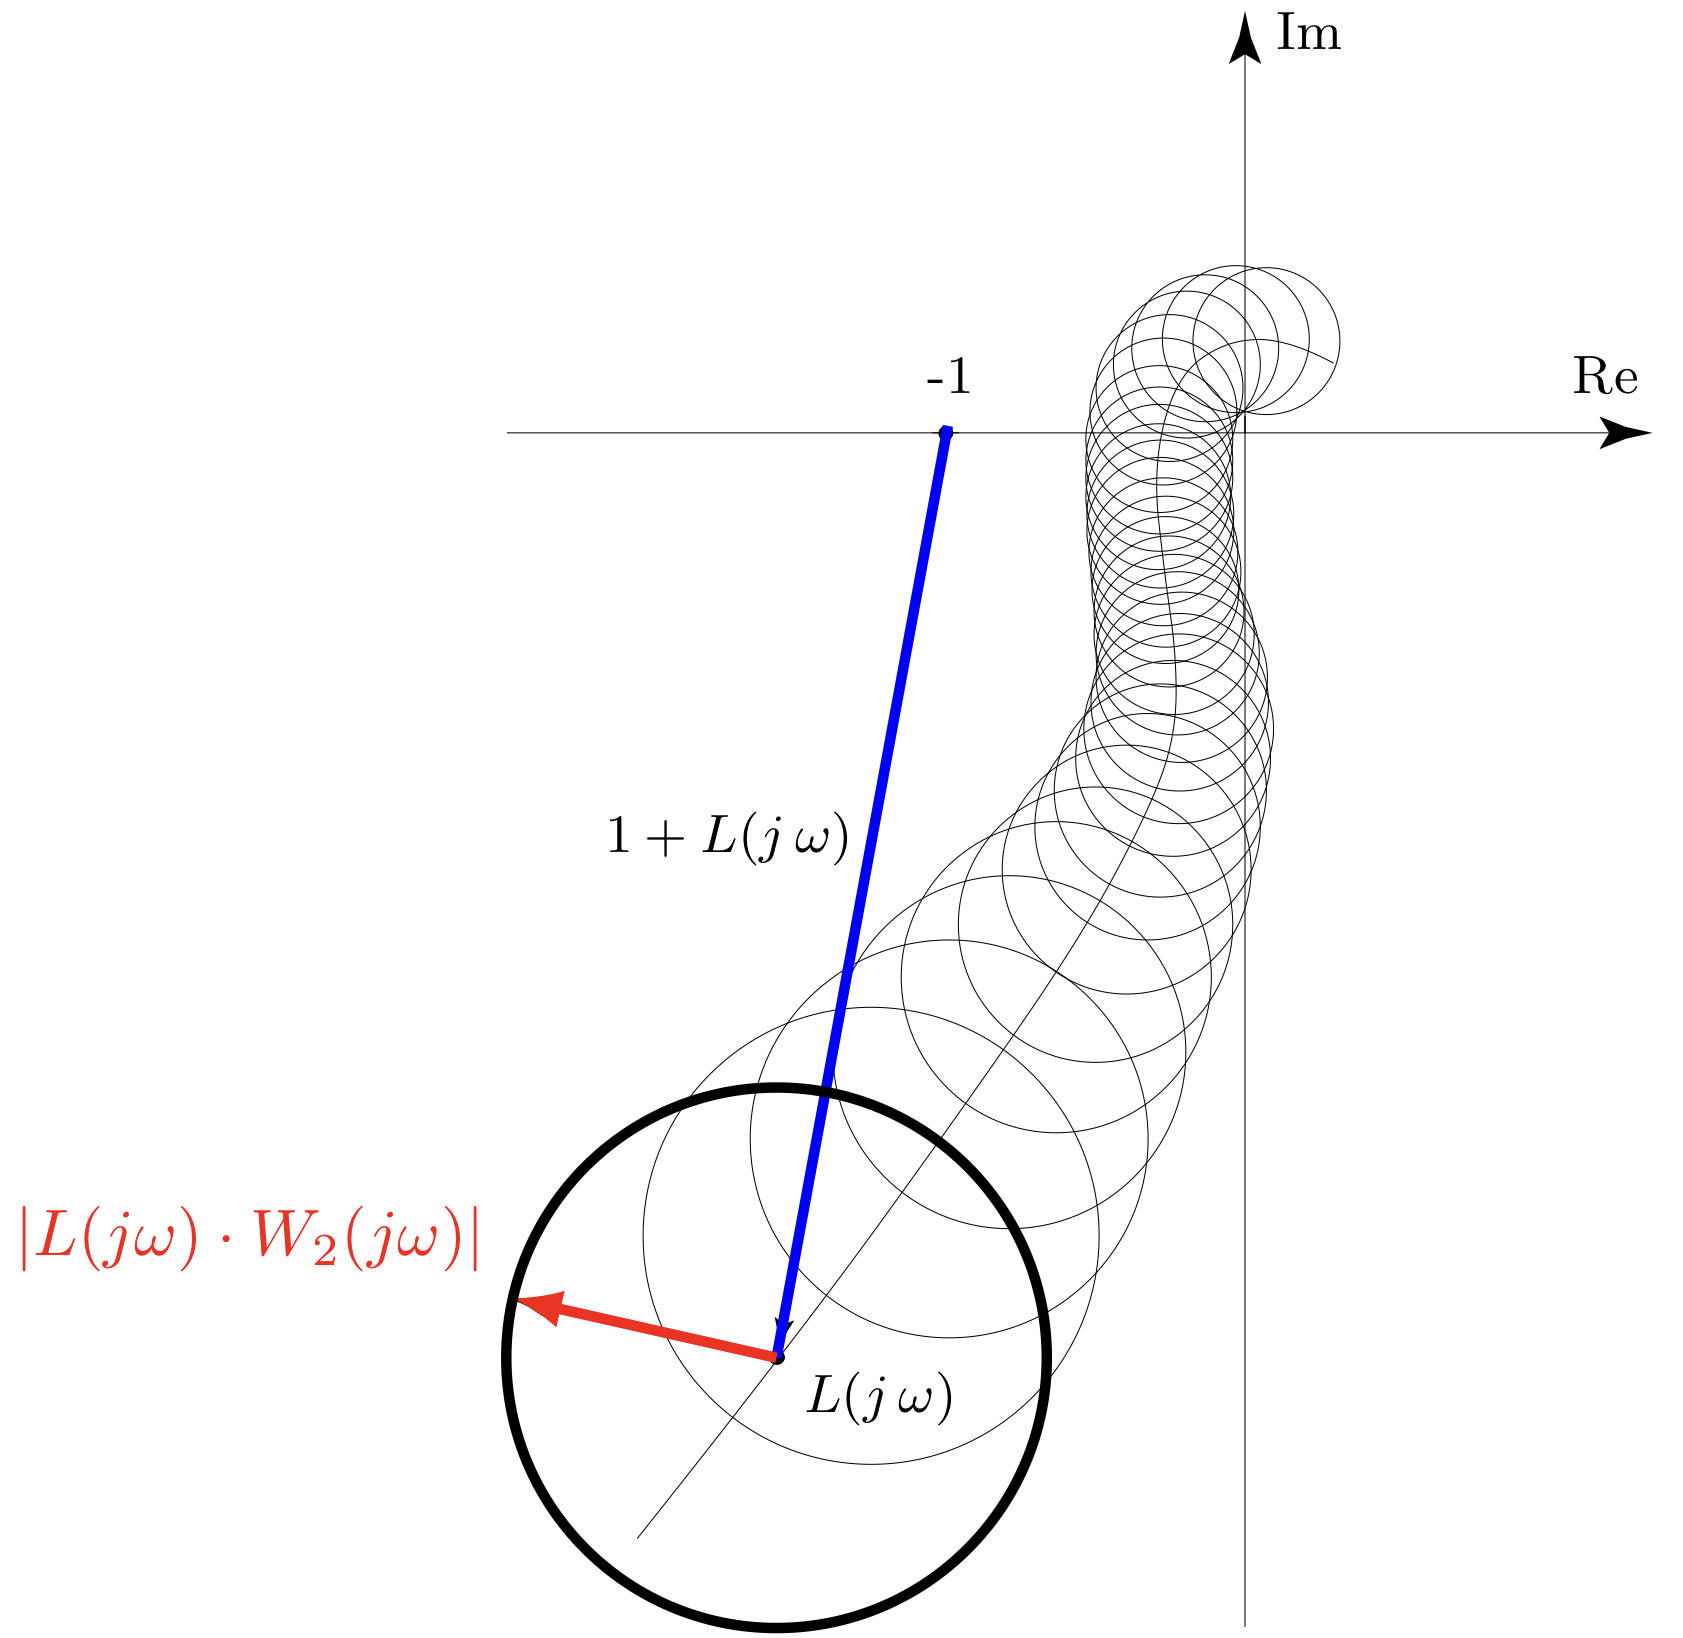
\includegraphics[width= 0.5\linewidth]{03/rob_nyquist.jpeg}
    \end{figure}
    
    Der rote Radius darf nicht grösser werden als der blaue Abstand vom Punkt $(-1 + j0)$ um zusätzliche Umrundungen vom krit. Punkt zu verhindern.
    
\subsection{Multiplikative Spezifikation von \textit{S(s)}}
    Wir wünschen eine betragsmässig kleine Sensitivität um Störungsunterdrückung und gutes reference tracking zu garantieren. Es ist daher sinnvoll den Betrag $|S(s)|$ frequenzabhängig zu limitieren (Disturbances nicht bei allen Frequenzen gleich relevant).
    
    \subsubsection{Nominelle Regelgüte}
        Um die Sensitivität zu Betragsmässig zu begrenzen wird eine rationale TF $W_1(s)$ eingeführt, wobei gelten muss:
        \begin{equation*}
        \colorboxed{red}{
        \begin{aligned}
            \| S(s)\cdot W_1(s)\|_{\textcolor{red}{\infty}} < 1 &\Rightarrow |S(\jw)| < |W_1^{-1}(\jw)|\\
            |W_1(\jw)| &< |1 + L(\jw)|
        \end{aligned}
        }
        \end{equation*}
        
        Die geometrische Interpretation von $W_1(s)$ ist, dass $L(\jw)$ nicht in einen um $(-1 + j0)$ zentrieren Kreis mit Radius $|W_1(\jw)|$ eintreten darf.
    
    \subsubsection{Konstruktion der nominellen Regelgüte}
        $W_1(s)$ kann als Lowpass-Filter konstruiert werden:
        \begin{align*}
            W_1(s) &= k\cdot\frac{\tau\cdot s + 1}{\alpha\cdot\tau\cdot s + 1}, \quad k > 1,\, \alpha > k\\
            \tau^2 &= \frac{k^2 - 1}{\omega_1^2\cdot(\alpha^2-k^2)}, \quad |W_1(\jw_1)| = 1
        \end{align*}
        
        \begin{figure}[H]
            \centering
            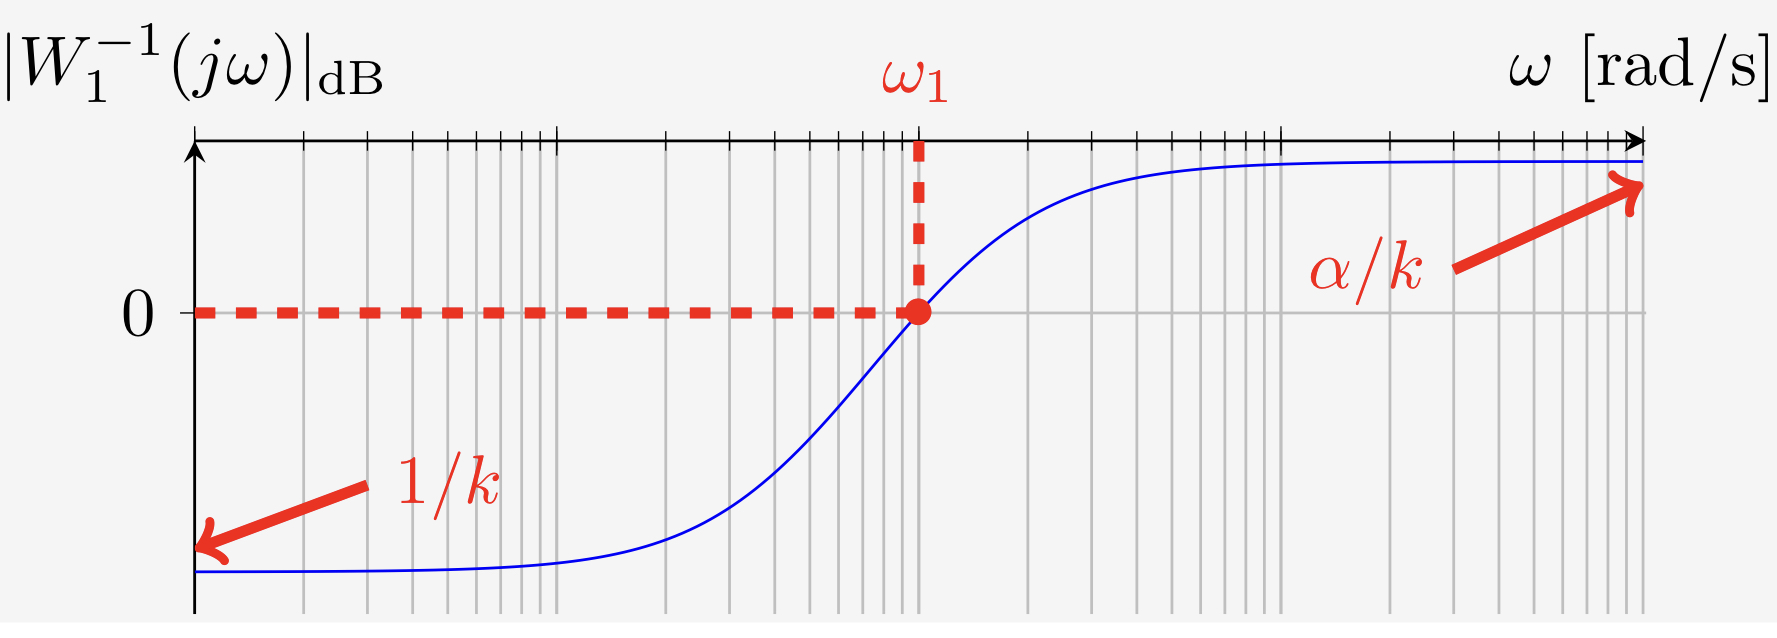
\includegraphics[width = 0.8\linewidth]{images/03/W_1.jpeg}
            \caption{$|W_1^{-1}|_\textnormal{dB}$ in blau. Einstellbare Grössen in rot.}
        \end{figure}

